\chapter{Reactor Mass Model} \label{ch:mass_model}
The reactor mass model was created as a submodel of the power cycle mass
model. The reactor mass model was designed to take flow property inputs (T, P,
$\dot{m}$) and constrain a reactor concept that is both coolable, and critical
after 10 years of full power operation. The reactor model was developed in
Python. The attribute of interest is the mass of
the valid concept, but other useful values such as geometry, fuel fraction,
and fluid-flow paramters are available from the solver. Before the mass model
could be built, some important design decisions needed to be made.


\section{Thermal Hydraulic Theory}
    The first considered constraint of a valid reactor design was coolability. The reactor must
not melt and the integrity of the fuel must be maintained for the duration of
the mission. To ensure the thermal hydraulic validity of a chosen design, 
    1D heat transfer and bulk-averaged fluid flow calculations were performed. The 1D
heat transfer and fluid equations were coupled with analytical flux shape
factors from nuclear engineering literature to determine the maximum extractable
thermal power for each reactor design. A 1D resistance network is used to
determine the maximum thermal generation for a given core design and temperature
drop between fuel meat and coolant. An iterative solving scheme was developed to
converge the heat transfer and fluid flow equations.

\subsection{Flow Properties}
All flow properties were axially averaged between their inlet and outlet values.
The inlet and outlet flow conditions, thermal power, and mass flow rate are
dictated by the power cycle configuration and requirements. Property tables for
both CO2 and H2O coolants as a function of pressure and temperature were 
generated using EES and interpolated using SciPy's 2D interpolation functions
\citep{scipy}, \citep{EES_citation}.
The interpolated properties included: thermal conductivity [W/m-K], density
[kg/m$^3$], viscosity [kg/m-s], and specific heat [J/kg-K].

\subsection{Core Geometry}

Important core geometry parameters were calculated. The coolant flow area,
average distance of conduction in the fuel, volume fraction of cladding in
coolant, number of coolant channels, convection surface area, LD, and the cross
sectional area for conduction in the fuel. The core radius is set by a critical
radius constraint dependent on the fuel fraction. This will be discussed in a
later section.

Fuel area and volume is derived from the core radius and fuel fraction. Where
$AR$ is the core aspect ratio.

\begin{equation}
    A_{fuel} = frac_{fuel}*r_{core}^2*\pi
\end{equation}
\begin{equation}
    V_{fuel} = A_{cool}*AR*r_{core}
\end{equation}

The fraction of cladding in the coolant is derived from the coolant channel
radius and cladding thickness.

\begin{equation}
    frac_{clad} = \frac{(r_{channel} + t_{clad})^2 - r_{channel}^2}{r_{channel}^2} 
\end{equation}

In a similar vein, coolant flow area is derived from the core radius, cladding
fraction, and fuel fraction

\begin{equation}
    A_{cool} = (1-frac_{fuel})*(1-frac_{clad})*r_{core}^2*\pi
\end{equation}

\begin{equation}
    V_{cool} = A_{cool}*AR*r_{core}
\end{equation}

The number of coolant channels is derived from the area of each channel and the
core flow area.

\begin{equation}
    N_{channels} = \frac{A_{cool}}{(r_{channel} + t_{clad})^2 * \pi}
\end{equation}

The convection surface area is dervied from the channel radius, core length, and
number of channels.

\begin{equation}
    A_{conv} = 2*r_{channel}*\pi*r_{core}*AR*N_{channels}    
\end{equation}

The length over diameter is derived from the channel radius and core length.

\begin{equation}
    LD = \frac{r_{core}*AR}{2*r_{channel}}
\end{equation}

The average distance to conduction is derived from fuel area and number of
channels.

\begin{equation}
    R_{cond} = \frac{\sqrt{\frac{A_{fuel}}{N_{channels}}}}{2}
    \label{r_cond}
\end{equation}

The cross sectional area for conduction in the fuel was conservatively estimated
as the convection surface area. In reality, the cross-sectional area changes as
heat transfers from the center of the fuel meat to the coolant channels.


These are the important equations defining the 1D geometry for a coolable
reactor. Once the geometry has been defined, the flow conditions are modeled.

\subsection{Flow Equations}

Once the core geometry has been defined, the flow is characterized using
bulk-averaged flow conditions and the reactor geometry. The mass flux, coolant
velocity, Reynold's number, Nusselt number and average heat transfer
coefficients are calculated.

Mass flux is derived from flow area and the mass flow rate dictated by the power
cycle. Flow velocity can be calculate from mass flux and density.

\begin{equation}
    \dot{G} = \frac{\dot{m}}{A_{flow}}
\end{equation}

\begin{equation}
    v = \frac{\dot{G}}{\rho}
\end{equation}

The Reynold's number is derived from flow velocity, density, viscosity, and the
characteristic flow length (channel diameter, D).

\begin{equation}
    Re = \frac{\rho v D}{\mu}
\end{equation}

The Nusselt number is calculated using the same correlations as EES. Laminar,
turbulent, and transitional flows are all treated differently.

The average heat transfer coefficient is derived from the Nusselt number and
thermal conductivity of the fluid.

\begin{equation}
    \bar{h} = \frac{Nu k_{cool}}{D}
\end{equation}

\subsection{1D Thermal Generation Modeling}

With a fully defined geometry and fully characterized flow, the maximum thermal
output of the core is calculated. The maximum generation (at the center of the
core) is calculated using a 1D resistance network. The three resistances in the
network are: conduction in the fuel, conduction in the clad, and convection from
the clad to the coolant. Gap and interface resistances were ignored.

Resistance to conduction in the fuel was approximated as plane wall conduction.
\begin{equation}
    R_{fuel} =  \frac{R_{cond}}{k_{fuel}A_{cond}}
\end{equation}

\begin{equation}
    R_{clad} = log(1+\frac{t_{clad}}{r_{channel}})
\end{equation}

\begin{equation}
    R_{conv} = \frac{1}{2\bar{h}r_{channel}L\pi N_{channels}}
\end{equation}

The maximum heat transfer rate at the fuel centerline was derived from the
resistance network and the temperature drop. The temperature drop was determined
by the maximum fuel temperature (estimated to be half the melting temperature of
the fuel) and the bulk coolant temperature.

\begin{equation}
    Q^{'''}_{max} = \frac{dT}{R_{fuel} + R_{clad} + R_{conv}}
\end{equation}

Finally, the thermal generation at fuel centerline is scaled by the axial and
radial flux profiles to account for the cosine and bessel function shapes of the
flux. The scaling factor was taken from El-Wakil's Nuclear Heat Transport
\citep{heat_trans_wakil}.

\begin{equation}
    Q_{gen} = Q^{'''}_{max} * 0.275
\end{equation}

\subsection{1D Thermal Hydraulic Calcuations}
    The governing equations above describe a coolable
reactor design. A Python code was written to solve the system of equations
defining the geometry, flow conditions, and 1D heat transfer in the reactor. The
code utilizes Scipy's optimization package. The 'optimize\_scalar' function is
used to guess fuel fraction values. For each fuel fraction, the above equations
are used to determine $Q_{gen}$, an error exists between $Q_{gen}$ and the
required thermal reactor output dictated by the power cycle requirements. The
optimization function minimizes the squared difference between $Q_{gen}$ and the
thermal power requirements. When the solver converges on a fuel fraction, the
code returns a coolable reactor design. Since the core radius was set by a
critical radius constraint, this reactor is also neutronically valid for the
duration of the 10 year mission.

    The thermal hydrauilc code also calculates the mass of each reactor. This
mass includes fuel, cladding, coolant, reflector material and the pressure
vessel. The pressure vessel thickness was calculated as a function of pressure
and outer core radius (including the reflector) for stainless steel at \~700K
using an ASME vessel thickness standard. Equation \ref{eq:pv_thick} was used to
define the pressure vessel thickness. This correlation is a conservative
estimate for pressure vessels and is adequate to ensure the integrity of the
vessel.

\begin{equation}
    T_{vessel} = \frac{RP}{S + 0.6P}
    \label{eq:pv_thick}
\end{equation}

\section{Limiting Core Mass}
The limiting core mass for both reactor constraints was analyzed to ensure the
reactor mass model was calculating the minimum reactor mass. For each fuel
fraction (F) there exists two constraining core radii such that:

\begin{align}
    R_{coolable} = G(F) \\
    R_{critical} = H(F)
\end{align}

Each combination of radius and fuel fraction has a corresponding mass:

\begin{equation}
    M = M(R, F)
\end{equation}

The goal of the mass optimization was to find the minimum mass that satisfies
both constraints.

\begin{equation}
    min( M(R_{coolable}, F), M(R_{critical}, F) )
\end{equation}

To ensure the model was returning the minimum reactor mass, both limiting mass
cases were plotted as a function of fuel fraction. This analysis was done for a
fixed set of flow conditions and a fixed thermal power. Figure
\ref{fig:limiting_core_mass} shows the limiting core mass constraint as a
function of fuel fraction.

\begin{figure}[h]
    \centering
    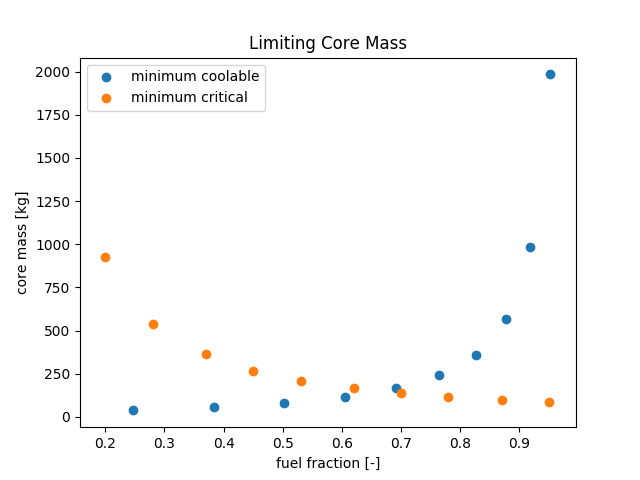
\includegraphics[width=5in]{../images/limiting_core_mass.png}
\caption{Limiting core mass constraints ensure mass-optimized reactor is found.}
\label{fig:limiting_core_mass}
\end{figure}

The reactor configuration calculated by the mass model is the intersection of
the critical core mass and the coolable core mass curves. The critical radius
constraint forces the reactor to be on the critical radius curve. The shape of
both curves ensures the intersection is the minimum mass reactor. For the
critical mass curve, any point below the curve does not meet the target
reactivity and any point above the curve exceeds the target reactivity. For the
coolable mass curve, any point below can not reject the required thermal heat
input and any point above is not reaching its thermal power potential. The
curves have opposite slopes, which means there exists no valid point on either
curve except for the intersection. Points above both lines represent valid
core designs, but are not the mass-optimized result.
